\HeaderQuote{If it had grown up, it would have made a dreadfully ugly child; but it makes rather a handsome pig, I think.}{Alice} 

\chapter{Problem generators}\label{ch:genprobleminstances} 

\FirstSentence{S}{ynthetic problem instances for } \JSP\ and \FSP\  will be used  throughout this dissertation. The  problem spaces are detailed in the \cref{sec:data:JSP,sec:data:FSP} for \JSP\ and \FSP, respectively. Moreover, a brief summary is given in \cref{tbl:data}.
Following the approach in \citet{Whitley}, difficult problem instances are not 
filtered out beforehand. %, although they will be specifically addressed in 
%\cref{ch:defdifficulty}. 
The problem spaces for \cref{Papers} are summarised in 
\cref{tbl:papers:problems}. Note, that the problem generators in 
\cref{InRu14,InRu15a,InRu15b} are the same as described here.

\begin{table}[b]
    \caption{\JSP\ and  \FSP\ problems spaces used in \cref{Papers}}
    \label{tbl:papers:problems}
    \noindent 
    \begin{minipage}{\textwidth}\centering
    {\setlength{\tabcolsep}{3pt}
    \begin{tabular}{c l l l l}\toprule
      Paper & Problem & $I=[u_1,u_2]$\footnote{Processing times are uniformly
        distributed from an interval $I=[u_1,u_2]$, i.e., 
        $\vec{p}\sim\mathcal{U}(u_1,u_2)$.} & size ($n\times m$) & name \\ 
        \midrule
      \ref{InRu11a} & \JSP & $[1,100], [50,100]$ & $6\times6$ & j.rnd, j.rndn\\
      \ref{InRu12} & \JSP & $[1,200]$ & $6\times 6$ & j.rnd \\
      \ref{InRu14} & \JSP, \FSP & $[1,99],[45,55]$ & $6\times5,10\times10$ & 
      j.rnd, j.rndn, f.rnd, f.rndn, f.jc\\
      \ref{InRu15a} & \JSP & $[1,99],[45,55]$ & $6\times5$ & j.rnd, j.rndn\\
      \ref{InRu15b} & \JSP, \FSP & $[1,99],[45,55]$ & $10\times10$ & 
      j.rnd, j.rndn, f.rnd\\
      \ref{InRu15c} & \JSP, \FSP & $[1,99],[45,55]$ & $6\times5,10\times10$ & 
      j.rnd, j.rndn, f.rnd\\
      \bottomrule
    \end{tabular}}
    \end{minipage}
\end{table}


Although real-world instances are desirable, unfortunately they are scarce. 
Hence in some experiments (mainly in \cref{ch:orlibrobust}), problem instances 
from OR-Library maintained by \citet{ORlibrary} will be used as benchmark 
problems. They are detailed in \cref{sec:data:orlib}. 

It is noted, that some of the instances are also simulated, but the majority 
are based on real-world instances, albeit sometimes simplified. 
%\citet{Panwalkar77} reports an extensive survey of 36 research papers in scheduling, most experiments are based on simulated data, and its verification on real-world data would be desirable, but missing. 

\section{\Jsp}\label{sec:data:JSP}
Problem instances for \JSP\ are generated stochastically by fixing the number of jobs and machines and 
discrete processing time are i.i.d. and sampled from a discrete uniform distribution. % from the interval $I=[u_1,u_2]$, i.e., $\vec{p}\sim \mathcal{U}(u_1,u_2)$. 
Two different processing times distributions were explored, namely,
\begin{description}
	\item[\Jrnd] \jrnd{n}{m} \hfill \\ where $\vec{p}\sim\mathcal{U}(1,99)$;
	\item[\Jrndn] \jrndn{n}{m} \hfill \\ where $\vec{p}\sim\mathcal{U}(45,55)$.
\end{description}
The machine ordering is a random permutation of all of the machines in the \jsp. 
For each \JSP\ class $N_{\train}$  and $N_{\test}$ instances were 
generated for training and testing, respectively. Values for $N$ are given in 
\cref{tbl:data}. 

Although in the case of \jrnd{n}{m}\ this may be an excessively large range for 
the uniform distribution, it is however, chosen in accordance with the 
literature \citep{Demirkol98} for creating synthesised $Jm||C_{\max}$ problem 
instances. 

In order to inspect the impact of any slight change within the problem spaces, 
two mutated versions were created based on \jrnd{n}{m}, namely, 
\begin{description}
	\item[\JrndJ] \jrndJ{n}{m} \hfill \\ where the first job, $J_1$, is always twice as long as its random counterpart, i.e.,\linebreak
	$\tilde{p}_{1a}=2\cdot p_{1a}$, where $p\in$\jrnd{n}{m}, for all $M_a\in\mathcal{M}$. 
	\item[\JrndM] \jrndM{n}{m} \hfill \\ where the first machine, $M_1$, is always twice as long as its random counterpart, i.e.,\linebreak
	$\tilde{p}_{j1}=2\cdot p_{j1}$, where $p\in$\jrnd{n}{m}, for all $J_j\in\mathcal{J}$. 
\end{description}
Therefore making job $J_1$ and machine $M_1$ bottlenecks for \jrndJ{n}{m} and 
\jrndM{n}{m}, respectively.

\citet{Hildebrandt2010} argue that the randomly generated problem 
instances aren't a proper representative for real-world long-term \jsp\   
applications, e.g., by the narrow choice of release-dates, yielding schedules 
that are overloading in the beginning phases. However, as stated in
\cref{ch:scheduling}, release-dates constraints won't be considered here.
In addition, w.r.t. the machine ordering, one could look into a 
subset of \JSP\ where the machines are partitioned into two (or more) sets, 
where all jobs must be processed on the machines from the first set (in some 
random order) before being processed on any machine in the second set, commonly 
denoted as $Jm|2\textrm{sets}|C_{\max}$ problems, but as discussed in 
\cite{orlib_swv} this family of \JSP\ is considered `hard' (w.r.t. relative 
error from best known solution) in comparison with the `easy' or 
`unchallenging' family with the general $Jm||C_{\max}$ set-up. % ath. 
%Holtsclaw96 vitnar í orlib_swv um easy-hard pælinguna
This is in stark contrast to \citet{Whitley} whose findings showed that 
structured $Fm||C_{\max}$ were much easier to solve than completely random 
structures. 
Intuitively, an inherent structure in machine ordering should be exploitable 
for a better performance.  However, for the sake of generality, a random 
structure is preferred as they correspond to difficult problem instances in the 
case of \JSP. Whereas, structured problem subclasses will be explored for 
\FSP.  

\section{\Fsp}\label{sec:data:FSP}
Problem instances for \FSP\  are generated using \citet{Whitley} problem 
generator.\footnote{Both code, written in \texttt{C++}, and problem instances 
used in their experiments can be found at: 
\url{http://www.cs.colostate.edu/sched/generator/}}
There are two fundamental types of problem classes: non-structured versus 
structured.

Firstly, there are two `conventional' random (i.e. non-structured) problem 
classes for \FSP\  where processing times are i.i.d. and uniformly distributed, 
\begin{description}
	\item[\Frnd]  \frnd{n}{m} \hfill \\
	where $\vec{p}\sim\mathcal{U}(1,99)$ whose instances are equivalent to \cite{Taillard1993}\footnote{\citeauthor{Taillard1993}'s generator is available from the OR-Library.};
	\item[\Frndn]  \frndn{n}{m} \hfill \\
	where $\vec{p}\sim\mathcal{U}(45,55)$.
\end{description}
In the \JSP\ context \frnd{n}{m}\ and \frndn{n}{m}\ are analogous to \jrnd{n}{m}\ and \jrndn{n}{m}, respectively.  

Secondly, there are three structured problem classes of \FSP\  which are modelled after real-world \emph{characteristics} in \fsp\ manufacturing, namely, 
\begin{description}
	\item[\Fjc] \fjc{n}{m} \hfill \\
	where $\vec{p}$ is dependent on job index, however, independent of 
	machine index. 
	\item[\Fmc]  \fmc{n}{m} \hfill \\
	where $\vec{p}$ is dependent on machine index, however, independent of 
	job index. 
	\item[\Fmxc]  \fmxc{n}{m} \hfill \\
	where $\vec{p}$ is dependent on machine and job indices. 
\end{description} 
In all cases, the (job, machine or mixed) correlation can be of degree 
$0\leq\alpha\leq1$. 
When $\alpha=0.0$ the problem instances closely correspond to \frnd{n}{m}, 
hence the degree of $\alpha$ controls the transition of random to structured. 
Let's assume $\alpha=1$.

An example of distribution of processing times are depicted in 
\cref{fig:fsp:structure}, where machine indices are on the horizontal axis, job 
indices are shape-coded, and their corresponding processing times, $p_{ja}$, 
are on the vertical axis.

\begin{figure}\centering 
  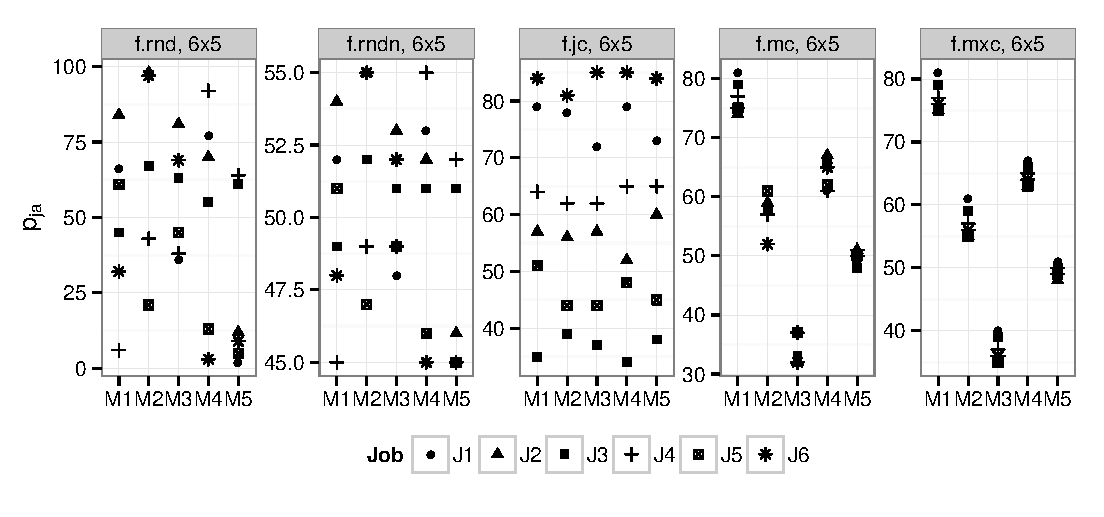
\includegraphics[width=\textwidth]{proctimes.pdf}
  \caption[Examples of job processing times of different \FSP\ structures 
  ]{Examples of job processing times for $6\times5$ of different \FSP\ 
  structures}
  \label{fig:fsp:structure}
\end{figure}

For each \FSP\  class $N_{\train}$  and $N_{\test}$ instances were 
generated for training and testing, respectively. Values for $N$ are given in 
\cref{tbl:data}. 

\begin{table}[t]\centering
	\caption{Problem space distributions used in experimental studies. 
    %Note, problem instances are synthetic and each problem space is i.i.d.
  }\label{tbl:data}
	{\renewcommand{\arraystretch}{1.5}
		\begin{tabular}{llcccl}\toprule
			& name           & size ($n\times m$) & $N_{\train}$ & 
			$N_{\test}$ & note                          
			\\ \midrule
			\multirow{8}{*}{\rot{\JSP}}
			& \jrnd{6}{5}   &$6\times5$ & 500 & 500 & random \\
			& \jrndn{6}{5}  &$6\times5$ & 500 & 500 & random-narrow \\
			& \jrndJ{6}{5}  &$6\times5$ & 500 & 500 & random with job variation \\
			& \jrndM{6}{5}  &$6\times5$ & 500 & 500 & random with machine variation \\
      & \jrnd{10}{10} &$10\times10$& 300 & 200 & random \\
			& \jrndn{10}{10}&$10\times10$& 300 & 200 & random-narrow \\ 
      &\jrndJ{10}{10} &$10\times10$& 300 & 200 & random with job variation\\
      &\jrndM{10}{10} &$10\times10$& 300 & 200 & random with machine variation\\
			\midrule
			\multirow{6}{*}{\rot{\FSP}}
			& \frnd{6}{5}  & $6\times5$ & 500 & 500 & random \\ 
			& \frndn{6}{5} & $6\times5$ & 500 & 500 & random-narrow \\ 
			& \fjc{6}{5}   & $6\times5$ & 500 & 500 & job-correlated \\ 
			& \fmc{6}{5}   & $6\times5$ & 500 & 500 & machine-correlated \\ 
			& \fmxc{6}{5}  & $6\times5$ & 500 & 500 & mixed-correlation \\ 
			& \frnd{10}{10}& $10\times10$ & 300 & 200 & random \\ 
			\bottomrule
		\end{tabular}}
\end{table}

\section{Benchmark problem suite}\label{sec:data:orlib}
A total of 82 and 31 benchmark problems for \JSP\ and \FSP, respectively, were 
obtained from the Operations Research Library (OR-Library) maintained by 
\citet{ORlibrary} and summarised in \cref{tbl:data:orlib}. 
Given the high problem dimensions of some problems, the optimum is not known, 
hence in those instances \cref{eq:rho} will be reporting  deviation from the 
latest best known solution (BKS) from the literature, reported by 
\citet{Jain99,orlibJSP}, and for \FSP\  consult \citet{orlibFSP}.

\subsection*{\Jsp\ OR-Library}
\citet{orlib_ft} had one of the more notorious benchmark problems for \JSP, and 
computationally expensive. However, now these instances have been solved to 
optimality. 
Similar to the synthetic \JSP\ problem spaces discussed earlier, 
\citet{orlib_abz} introduce five \JSP\ instances with a random machine ordering 
and processing times $\vec{p}\sim\mathcal{U}(50,100)$, for  dimensions 
$10\times10$ and $20\times15$. 
Likewise, \citet{orlib_yn} consists of four $20\times20$ random 
problem instances, where $\vec{p}\sim\mathcal{U}(10,50)$.
\citet{orlib_swv} introduce a set of \JSP\ problems where 
$\vec{p}\sim\mathcal{U}(1,100)$. There are a total of five problems in four 
dimension classes 
\begin{enumerate*}
  \item $20\times10$ %(\texttt{swv01-swv05})
  \item $20\times15$ %(\texttt{swv06-swv10})
  \item $50\times10$ %(\texttt{swv11-swv15})
  \item $50\times10$ %(\texttt{swv16-swv20})
\end{enumerate*}
Where the first three classes are considered `{hard}' and the last one as 
`{easy}'. Easy problems are ones corresponding to random machine ordering, 
whereas hard problems are partitioned in such a way the jobs must be processed 
on the first half of the machines before starting on the second half, i.e., 
$Jm|\text{2sets}|C_{\max}$.
\citet{orlib_orb} introduced ten problem instances of $10\times10$ \JSP\ where 
generated such that the machine ordering was chosen by random users in order to 
make them `difficult.' Moreover, the processing times were drawn at random, 
and the distribution that had the greater gap between its optimal value and 
standard lower bound was chosen. 

\subsection*{\Fsp\ OR-Library}
For the \FSP\ benchmarks, \citet{orlib_hel} introduces two deterministic 
instances based on `many-machine version of book-printing,' where processing 
times for $n\in\{20,100\}$ jobs and $m=10$ machines are relatively short, 
i.e., $p_{ja}\in\{0,..,9\}$. \citet{orlib_car} however, comprises of eight 
problems (of various dimension) where there is high variance in processing 
times, presumably $\vec{p}\sim\mathcal{U}(1,1000)$. 
\citet{orlib_rec} argues that completely random problem instances are unlikely 
to occur in practice. However, only the random instances they used (type C) are 
reported in the OR-Library, for a total of 42 problem instances with processing 
times following a uniform distribution, $\vec{p}\sim\mathcal{U}(1,100)$, of 
dimensions varying from $20\times5$ to $75\times20$, although \cite{orlibFSP} 
omitted \ProblemSpace[75 \times 20]{reC} instances in their comparison.

\begin{table}\centering
\noindent
\begin{minipage}{\textwidth}
  \caption{Benchmark problems from OR-Library used in experimental studies.}
  \label{tbl:data:orlib}
  \begin{tabular}{llrrll}\toprule
    & name & $n\times m$ & $N_{\test}$ & note & shorthand  \\
    \midrule \multirow{6}{*}{\rot{\JSP}}
    &\ProblemSpace{ft} & various &  3 &\citet{orlib_ft} & 
    \texttt{ft06,ft10,ft20}\\
    &\ProblemSpace{la} & various & 40 &\citet{orlib_la} & 
    \texttt{la01-la40}     \\
    &\ProblemSpace{abz}& various &  5 &\citet{orlib_abz}& 
    \texttt{abz05-abz09}   \\
    &\ProblemSpace{orb}& $10\times10$& 10 &\citet{orlib_orb}& 
    \texttt{orb01-orb10}\\
    &\ProblemSpace{swv}& various & 20 &\citet{orlib_swv}&\texttt{swv01-swv20}\\
    & \ProblemSpace{yn} & $20\times20$& 4  &\citet{orlib_yn} & 
    \texttt{yn01-yn04}\\
    \midrule \multirow{3}{*}{\rot{\FSP}}
    &\ProblemSpace{car}& various &  8 & \citet{orlib_car} & \texttt{car1-car8} 
    \\
    &\ProblemSpace{hel}& various &  2 & \citet{orlib_hel} & \texttt{hel1,hel2}  
    \\
    &\ProblemSpace{reC}& various & 21 & \citet{orlib_rec}\footnote{Only 
    odd-numbered
        instances in \texttt{rec01-rec42} are given, since the even-numbered 
        instances are obtained from the previous instance by just reversing the 
        processing order of each job; the optimal value of each odd-numbered 
        instance and its even-numbered counterpart is the same.}  
    & \texttt{reC01-reC42}\\
    \bottomrule
  \end{tabular}
\end{minipage}
\end{table}
